\renewcommand{\baselinestretch}{2} \small\normalsize
\chapter{Multistatic RF Sensor Networks}
Analysis of RADAR systems in maritime environments is complicated by the fact that the ocean does not generally provide a smooth or uniform surface to work with. Altitude variations change the aspect angle for multipath bounces, induce wave blockage, and add clutter and spikes to the echo return \cite{skolnik_handbook}, \cite{blake_radar}, \cite{nathanson_radar}.

When we look at cases where the transmitter and receiver are no longer colocated, we have a bistatic system and the problem becomes even more difficult \cite{willis_bistatic}. As we add additional receivers or transmitters, the problem becomes multistatic. Of particular concern for this report is the case with a single transmitter and multiple receivers.

Figure \ref{ms_fig:1} shows the overall concept of a multistatic RF sensor network in a maritime environment. A single transmitter is illuminating a target and the echo signal is captured by a pair of receivers. In order to understand the probability of the target being detected by either receiver, we need to understand the statistics of the received signals.

\begin{figure}[H]
  \begin{center}
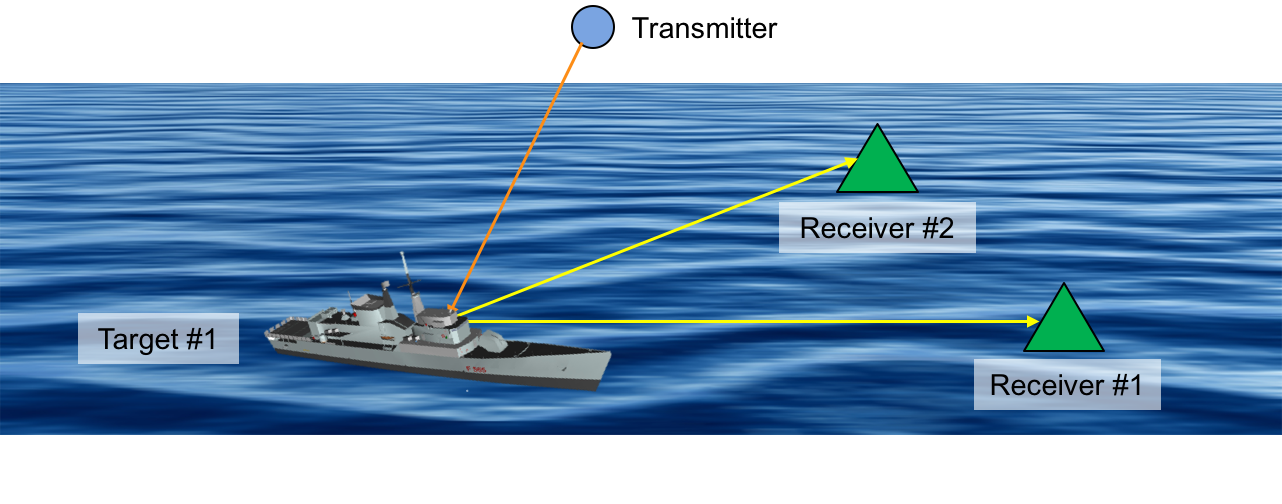
\includegraphics[width=5in]{../media/multistatic/ms_rf_concept.png}
  \end{center}
  \renewcommand{\baselinestretch}{1} \small\normalsize
  \begin{quote}
    \caption[Multistatic RF Sensor Networks Concept]{Multistatic RF Sensor Networks Concept\label{ms_fig:1}}
  \end{quote}
\end{figure}
\renewcommand{\baselinestretch}{2} \small\normalsize

For traditional monostatic RADAR systems, work done by Jess Marcum and Peter Swerling and provided statistical models for the fluctuating RADAR cross section (RCS) observed by targets \cite{richards_radar}. There are $4$ Swerling cases that are generally considered, using $2$ different decorrelation time lengths and $2$ different PDFs as shown in Table \ref{ms_tab:1}. 

\begin{table}[H]
  \begin{center}
      \renewcommand{\baselinestretch}{1} \small\normalsize
  \begin{quote}
    \caption[Swerling Fluctuating Target RCS Model Description]{Swerling Fluctuating Target RCS Model Description\label{ms_tab:1}}
  \end{quote}
  \begin{tabular} {|c | c | c |}
    \hline
  \bf{Case} & \bf{Decorrelation Time Length} & \bf{Chi-squared PDF Degree} \\ \hline
  1 &Long (Scan to Scan) &2 \\ \hline
  2 &Short (Pulse to Pulse) &2 \\ \hline
  3 &Long (Scan to Scan) &4 \\ \hline
  4 &Short (Pulse to Pulse) &4 \\ \hline
\end{tabular}
\end{center}
\end{table}
\renewcommand{\baselinestretch}{2} \small\normalsize
The Chi-squared PDF of degree $2$ covers the case with many randomly distributed small scatterers with none dominant and the Chi-squared PDF of degree $4$ covers the case with a single dominant scatterer and many small scatterers. These PDFs are shown in Figure \ref{ms_fig:2}.
\begin{figure}[H]
  \begin{center}
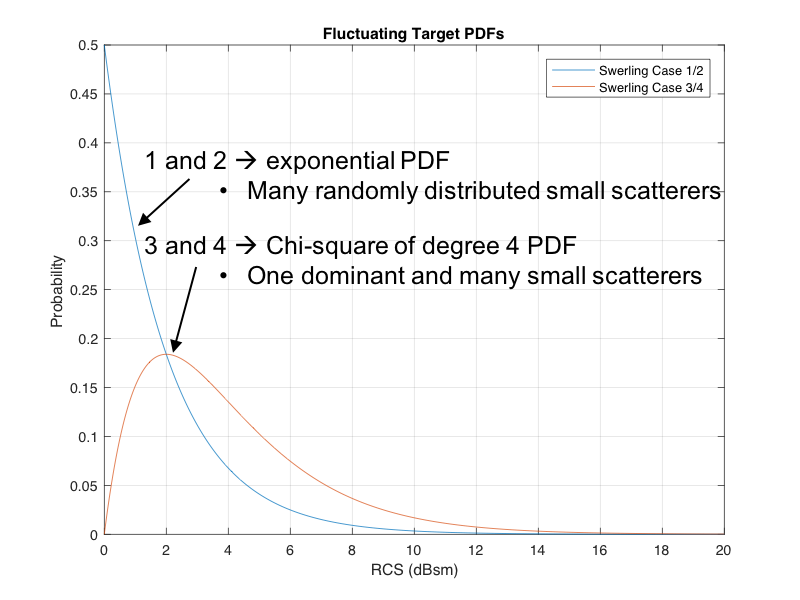
\includegraphics[width=4in]{../media/multistatic/swerling_pdfs.png}
  \end{center}
  \renewcommand{\baselinestretch}{1} \small\normalsize
  \begin{quote}
    \caption[Swerling Target Fluctuation Model PDFs]{Swerling Target Fluctuation Model PDFs\label{ms_fig:2}}
  \end{quote}
\end{figure}
\renewcommand{\baselinestretch}{2} \small\normalsize

The long decorrelation time covers the case where the target RCS can be considered constant over the time the RADAR performs a single scan and the short decorrelation time covers the case where the target RCS fluctuates on a pulse to pulse basis. A fluctuating signal can have a significant effect on the probability of dectection ($P_d$), as shown in Figure \ref{ms_fig:3}. This figure shows the $P_d$ as a function of Signal to Noise Ratio (SNR) for a nonfluctating target and a target following each of the $4$ Swerling cases and demonstrates that using the wrong PDF will results in errors in the computed $P_d$.
\begin{figure}[H]
  \begin{center}
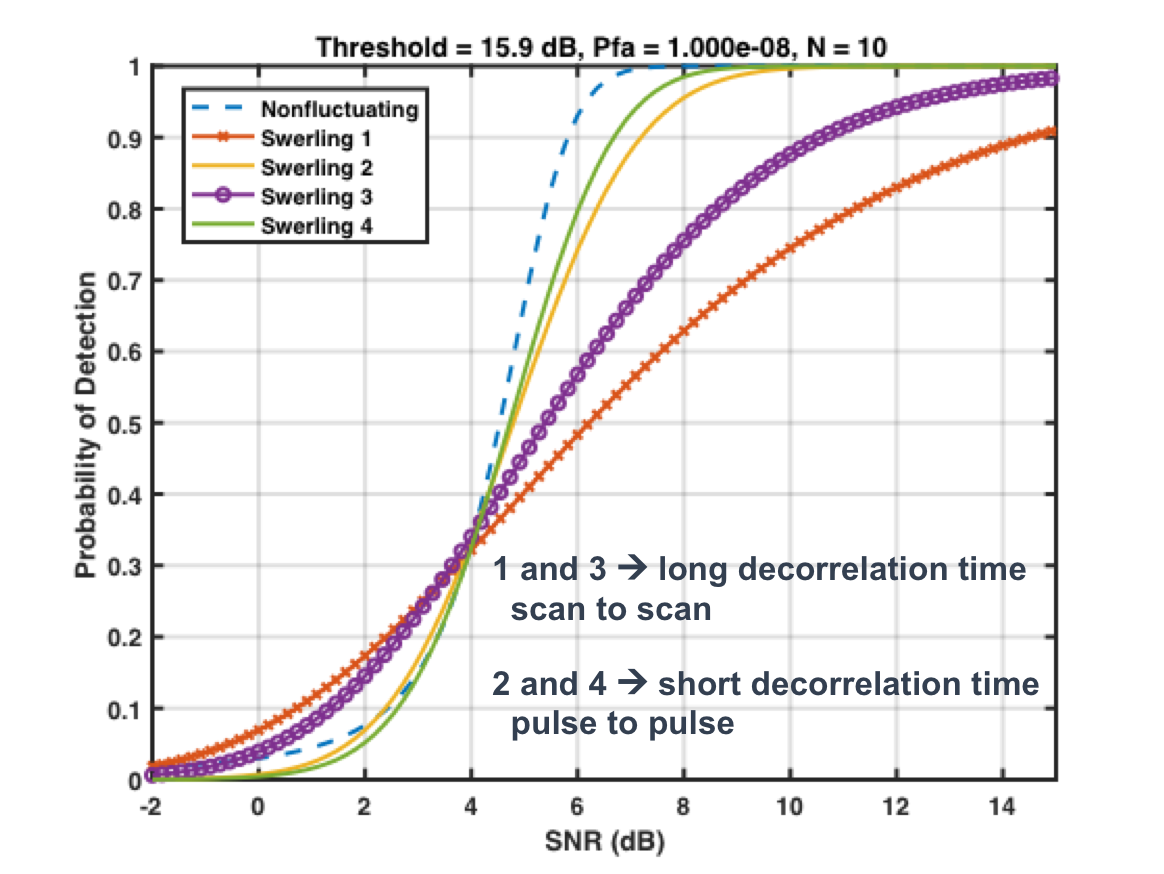
\includegraphics[width=4in]{../media/multistatic/swerling_pd.png}
  \end{center}
  \renewcommand{\baselinestretch}{1} \small\normalsize
  \begin{quote}
    \caption[Swerling Target Fluctuation Model Probability of Detection]{Swerling Target Fluctuation Model Probability of Detection\label{ms_fig:3}}
  \end{quote}
\end{figure}
\renewcommand{\baselinestretch}{2} \small\normalsize